\documentclass[a4paper, 12pt]{article}

\usepackage[utf8]{inputenc}
\usepackage[T2A]{fontenc}
\usepackage[english,russian]{babel}

\usepackage{amsmath,amsfonts,amssymb,amsthm,mathtools}
\usepackage{indentfirst}
\usepackage{ gensymb }
\mathtoolsset{showonlyrefs=true}
\usepackage{euscript}
\usepackage{mathrsfs}
\usepackage[left=2cm,right=2cm,top=2cm,bottom=2cm]{geometry}
\usepackage{graphicx}
\usepackage{wrapfig}
\usepackage{hyperref}
\usepackage[rgb]{xcolor}
\hypersetup{
colorlinks=true,
urlcolor=blue
}


\title{Лабораторная работа 2.4.1}
\author{Гисич Арсений Б03-109}
\date{2022}

\begin{document}

	\begin{center}
		{\large МОСКОВСКИЙ ФИЗИКО-ТЕХНИЧЕСКИЙ ИНСТИТУТ (НАЦИОНАЛЬНЫЙ ИССЛЕДОВАТЕЛЬСКИЙ УНИВЕРСИТЕТ)}
	\end{center}
	\vspace{5 cm}
	{\Large
		\begin{center}
			{\bf Лабораторная работа 2.4.1}\\[0.2 cm]
			Определение теплоты испарения жидкости
		\end{center}
	}
	\vspace{4 cm}
	\begin{flushright}
		{\Large Выполнил: \\
			\vspace{0.2 cm}
			Гисич Арсений \\
			\vspace{0.2 cm}
			Б03-109 \\}
	\end{flushright}
	\vspace{9 cm}
	\begin{center}
		Долгопрудный\\[0.1 cm]
		2022
	\end{center}
\thispagestyle{empty}

\section{Аннотация}

\par Цель работы: 1) измерение давления насыщенного пара жидкости при разной температуре; 2) вычисление по полученным данным теплоты испарения с помощью уравнения Клапейрона-Клаузиуса.

\section{Теоретические сведения}

\par Теплоту парообразования жидкостей можно измерить непосредственно при помощи калориметра. Такой метод, однако, не позволяет получить точных результатов из-за неконтролируемых потерь тепла, которые трудно сделать малыми. В настоящей работе для определения теплоты испарения применен
косвенный метод, основанный на формуле Клапейрона–Клаузиуса:
\begin{equation}\label{1}
\frac{dP}{dT} = \frac{L}{T(V_2 - V_1)}.
\end{equation}
Здесь $P$ — давление насыщенного пара жидкости при температуре $T$, $T$ — абсолютная температура жидкости и пара, $L$ — теплота испарения жидкости, $V_2$ — объем пара, $V_1$ — объем жидкости. Найдя из опыта $\frac{dP}{dT},\; T,\; V_2$ и $V_1$, можно определить $L$ путем расчета. Величины $L, \;V_2$ и $V_1$ в формуле (1) должны относиться к одному и тому же количеству вещества; мы будем относить их к одному молю.
\par В нашем приборе измерения производятся при давлениях ниже атмосферного. В этом случае задача существенно упрощается.
\par Обратимся теперь к $V_2$, котрое в дальнейшем будем обозначать просто $V$. Объём $V$ связан давлением и температурой уравнением Ван-дер-Ваальса:
\begin{equation}\label{2}
\left(P+\frac{a}{V^2}\right)(V-b)=RT.
\end{equation}
В уравнении Ван-дер-Ваальса величиной $b$ следует пренебречь. Пренебрежение членом $\frac{a}{V^2}$ по сравнению с $P$ вносит ошибку менее 3\%. При давлении ниже атмосферного ошибки становятся ещё меньше. Таким образом, при давлениях ниже атмосферного уравнение Ван-дер-Ваальса для насыщенного пара мало отличается от уравнения Клапейрона. Положим поэтому
\begin{equation}\label{3}
V=\frac{RT}{P}.
\end{equation}
Подставляя \eqref{3} в \eqref{1}, пренебрегая $V_1$ и разрешая уравнение относительно $L$, найдём
\begin{equation}\label{4}
L=\frac{RT^2}{P} \frac{dP}{dT} = -R\frac{d(lnP)}{d(1/T)}.
\end{equation}

\section{Методика измерений}

\parСхема установки изображена на рисунке 1. Наполненный водой резервуар 1 играет роль термостата. Нагревание термостата производится спиралью 2, подогреваемой электрическим током. Для охлаждения воды в термостате через змеевик 3 пропускается водопроводная вода. Вода в термостате перемешивается воздухом,
поступающим через трубку 4. Температура воды измеряетс
я термометром 5. В термостат погружен запаянный прибор 6 с исследуемой жидкостью. Над ней находится насыщенный пар (перед заполнением прибора воздух из него был откачан).
Давление насыщенного пара определяется по ртутному манометру,соединенному с исследуемым объемом. Отсчет показаний манометра производится при помощи микроскопа.


\begin{figure}[h!]
	\center{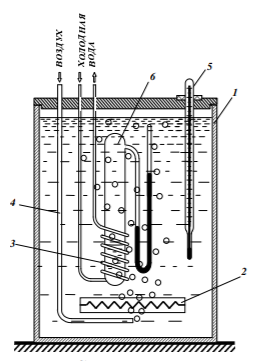
\includegraphics[scale=1.2]{lab_2_4_1_ust}}
	\caption{Схема установки для определения теплоты испарения}
\end{figure}

\section{Используемое оборудование}

\begin{enumerate}
    \item Термостат; $\delta_{\text{T}} = 0,1~\celsius$
    \item Герметичный сосуд, заполненый исследуемой жидкостью (водой);\par $\delta_{\text{шк}} = 0,02~\text{мм}$
    \item Отсчётный микроскоп; $\delta_{\text{шт}} = 0,05~\text{мм}$
\end{enumerate}

\section{Результаты измерений и обработка данных}

Начальные условия:\par

$\begin{aligned}
& h_1 = 6,8~\text{cм}\\
& h_2 = 4,98~\text{cм}\\
& \Delta{h} = 1,82~\text{cм}\\
& T_0 = 21~\celsius
\end{aligned}$\\[0,5 cm]

Результаты измерения давления при нагревании:

\begin{table}[h!]
\begin{tabular}{|c|c|c|c|c|c|c|c|c|c|}
\hline
$T, \celsius$ & 22      & 23      & 24      & 25      & 26     & 27      & 28      & 29      & 30     \\ \hline
$h_2, \text{cм}$ & 4,90    & 4,86    & 4,77    & 4,70    & 4,64   & 4,56    & 4,52    & 4,46    & 4,34   \\ \hline
$\Delta{h}, \text{cм}$ & 1,98    & 2,06    & 2,24    & 2,38    & 2,50   & 2,66    & 2,74    & 2,86    & 3,10   \\ \hline
$P, \text{Па}$  & 2639,34 & 2745,98 & 2985,92 & 3172,54 & 3332,5 & 3545,78 & 3652,42 & 3812,38 & 4132,3 \\ \hline
\end{tabular}
\end{table}

\begin{table}[h!]
\begin{tabular}{|c|c|c|c|c|c|c|c|c|c|}
\hline
31     & 32      & 33      & 34      & 35     & 36      & 37      & 38      & 39   & 40      \\ \hline
4,24   & 4,17    & 4,10    & 4,00    & 3,84   & 3,78    & 3,61    & 3,50    & 3,39 & 3,30    \\ \hline
3,30   & 3,44    & 3,58    & 3,78    & 4,10   & 4,22    & 4,56    & 4,78    & 5,00 & 5,18    \\ \hline
4398,9 & 4585,52 & 4772,14 & 5038,74 & 5465,3 & 5625,26 & 6078,48 & 6371,74 & 6665 & 6904,94 \\ \hline
\end{tabular}
\end{table}
\newpage

Результаты измерения давления при охлаждении:

\begin{table}[h!]
\begin{tabular}{|c|c|c|c|c|c|c|c|c|c|}
\hline
$T, \celsius$ & 22      & 23     & 24      & 25      & 26      & 27      & 28     & 29      & 30      \\ \hline
$h_2, \text{cм}$ & 4,91    & 4,84   & 4,80    & 4,70    & 4,63    & 4,52    & 4,44   & 4,36    & 4,30    \\ \hline
$\Delta{h}, \text{cм}$ & 1,96    & 2,10   & 2,18    & 2,38    & 2,52    & 2,74    & 2,90   & 3,06    & 3,18    \\ \hline
$P, \text{Па}$  & 2612,68 & 2799,3 & 2905,94 & 3172,54 & 3359,16 & 3652,42 & 3865,7 & 4078,98 & 4238,94 \\ \hline
\end{tabular}
\end{table}

\begin{table}[h!]
\begin{tabular}{|c|c|c|c|c|c|c|c|c|c|}
\hline
31     & 32     & 33      & 34      & 35      & 36     & 37      & 38      & 39      & 40      \\ \hline
4,24   & 4,14   & 4,06    & 3,92    & 3,83    & 3,74   & 3,62    & 3,53    & 3,36    & 3,30    \\ \hline
3,30   & 3,50   & 3,66    & 3,94    & 4,12    & 4,30   & 4,54    & 4,72    & 5,06    & 5,18    \\ \hline
4398,9 & 4665,5 & 4878,78 & 5252,02 & 5491,96 & 5731,9 & 6051,82 & 6291,76 & 6744,98 & 6904,94 \\ \hline
\end{tabular}
\end{table}

Полученные графики зависимости:\par

\begin{figure}[h!]
\begin{flushleft}
    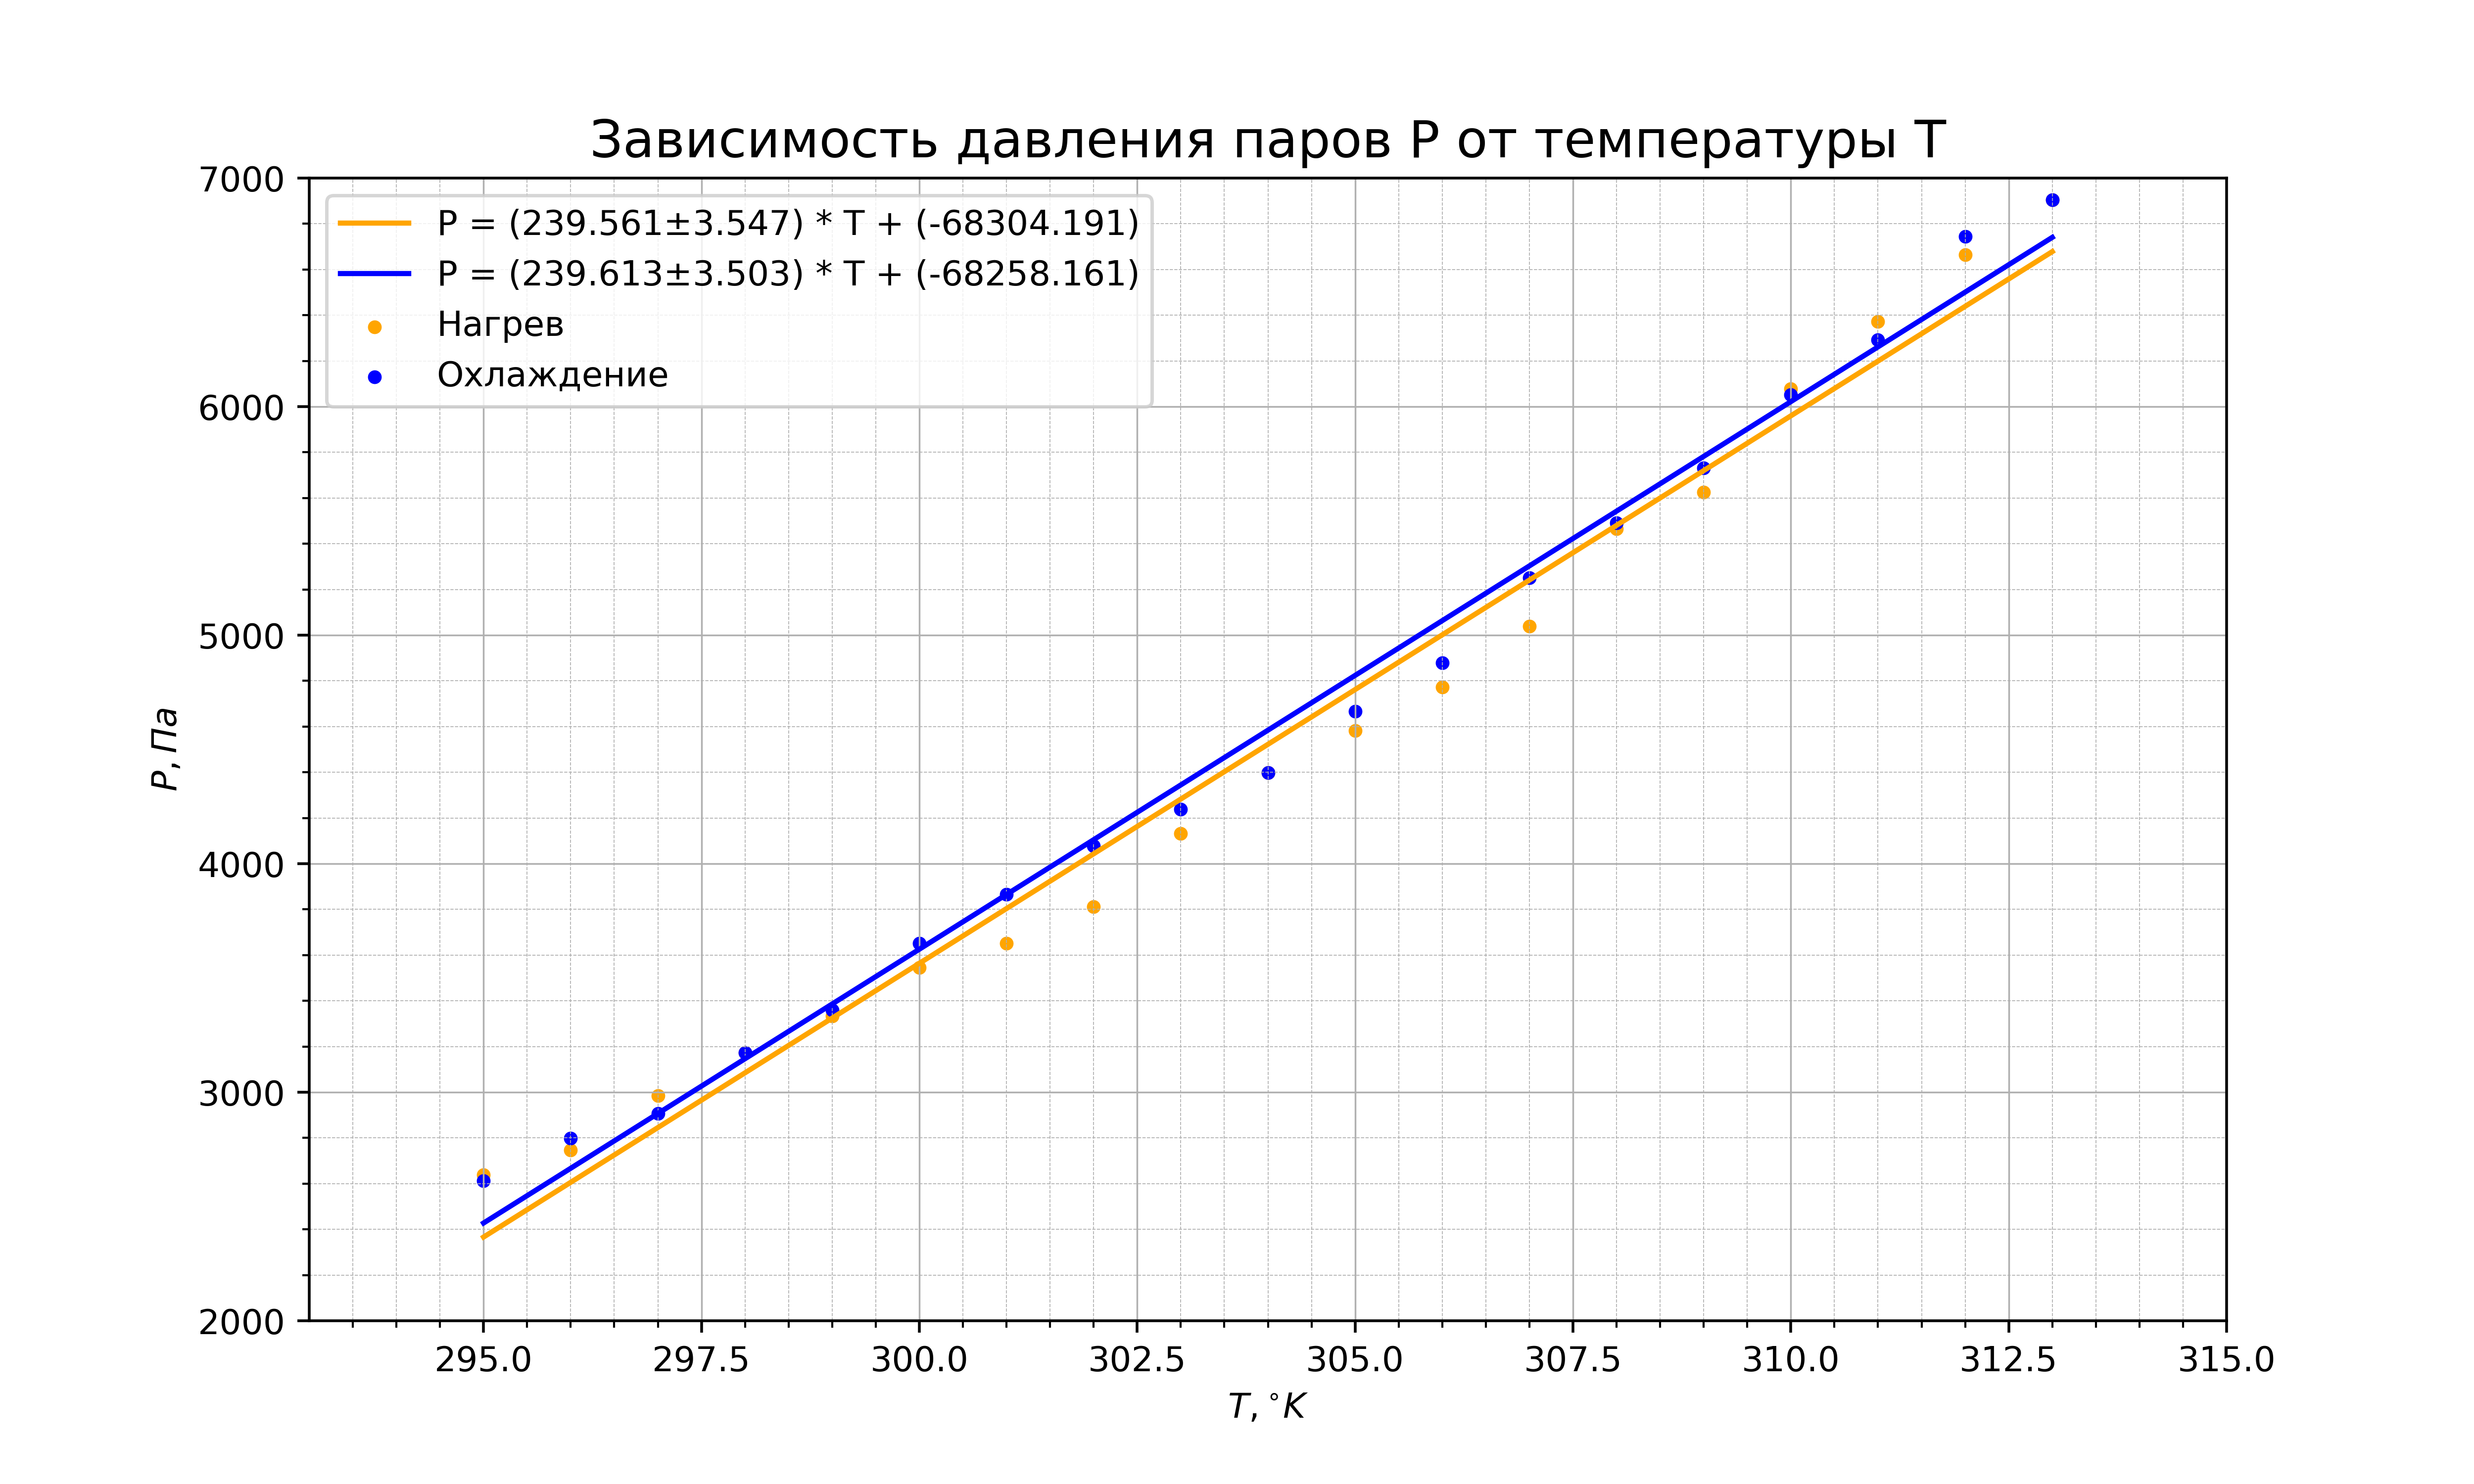
\includegraphics[scale=0.75]{2.4.1_1.png}
\end{flushleft}
\caption{}
\end{figure}

\begin{figure}[h!]
\begin{flushleft}
    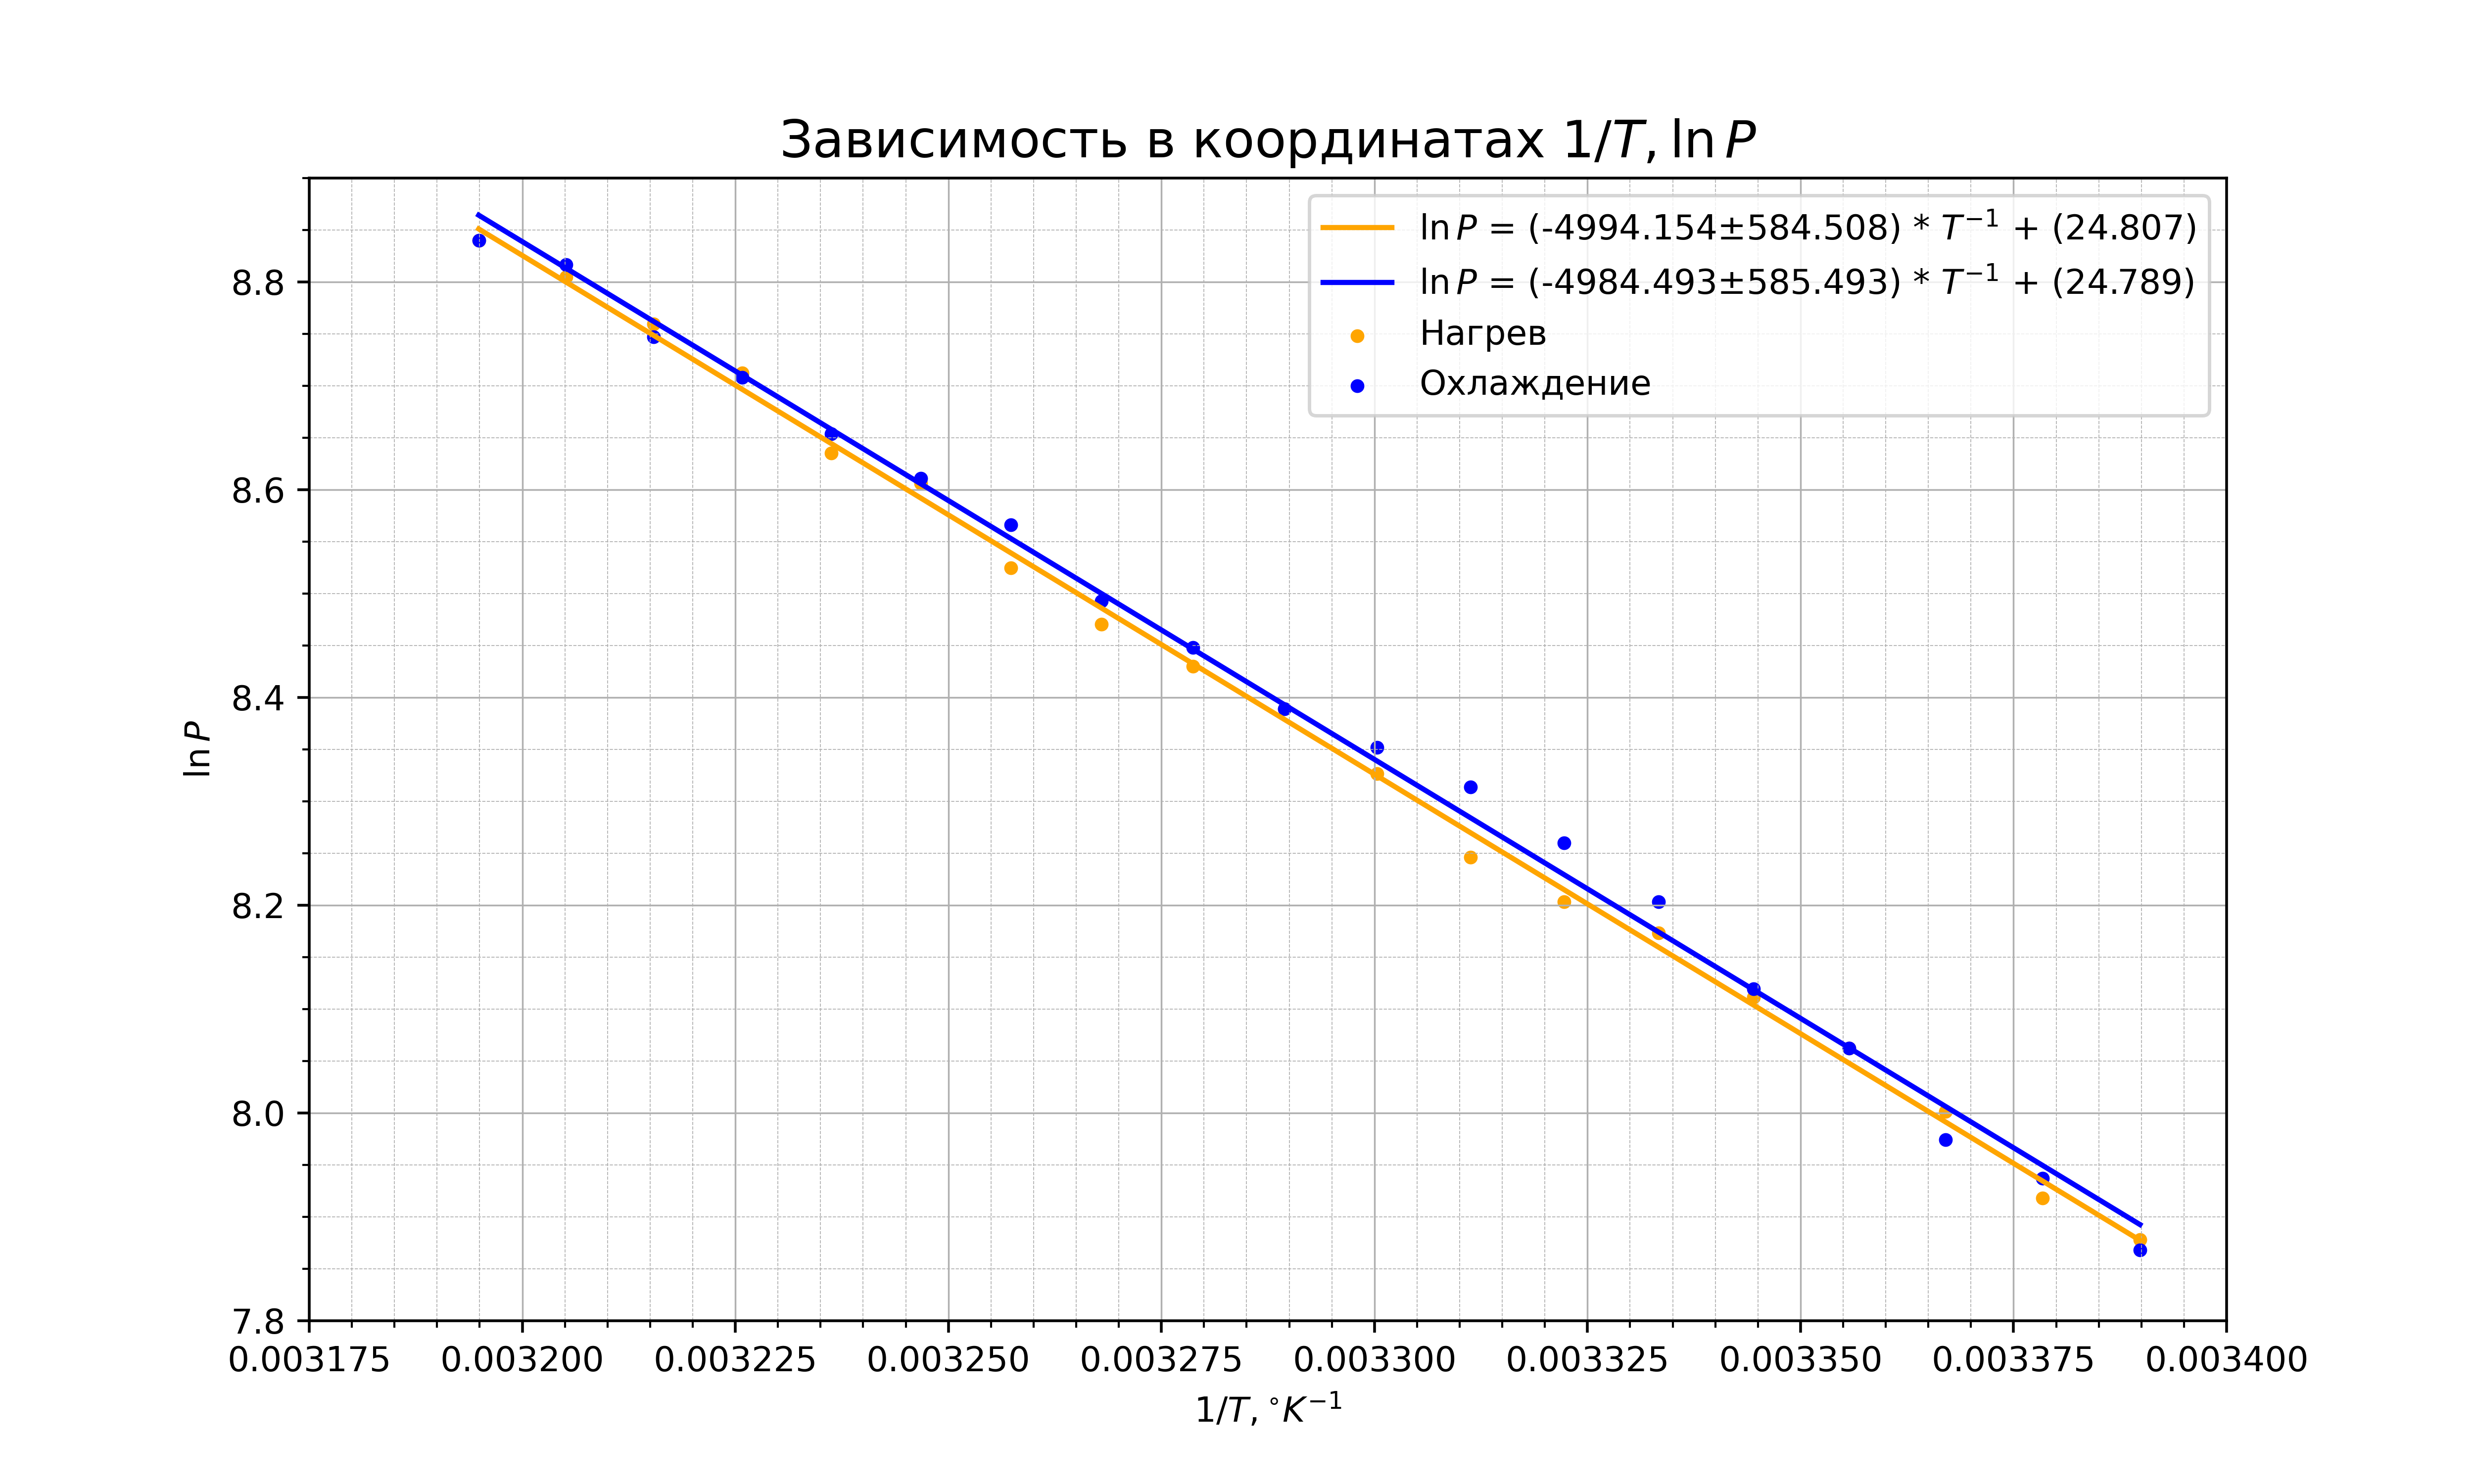
\includegraphics[scale=0.75]{2.4.1_2.png}
\end{flushleft}
\caption{}
\end{figure}

Полученные значения:

\begin{table}[h!]
\begin{tabular}{|c|cl|c|}
\hline
                          & \multicolumn{2}{l|}{Нагрев}        & Охлаждение    \\ \hline
$\frac{dP}{dT}$ & \multicolumn{2}{c|}{$239,56\pm3,55$} & $239,61\pm3,50$ \\ \hline
$\frac{d(\ln{P})}{d(1/T)}$ & \multicolumn{2}{c|}{$-4994,15\pm584,51$} & $-4984,49\pm585,49$ \\ \hline
\end{tabular}
\end{table}
\vspace{3 cm}
По формуле \eqref{4} находим $L$. Погрещность для первого способа определяется по формуле:

\begin{equation}\label{5}
\delta{_L} = \sqrt{\left(\frac{\delta{_P}}{P}\right)^2 + 4\left(\frac{\delta{_T}}{T}\right)^2 + \left(\frac{\delta{_{\frac{dP}{dT}}}}{\frac{dP}{dT}}\right)^2} \cdot L
\end{equation}

Полученные значения $L$:

\begin{table}[h!]
\renewcommand{\arraystretch}{1.8}
\begin{tabular}{|c|cl|c|}
\hline
                                    & \multicolumn{2}{c|}{Нагрев}       & Охлаждение   \\ \hline
$L, \frac{\text{МДж}}{\text{кг}}$ & \multicolumn{2}{c|}{$2,79\pm0,06$} & $2,75\pm0,06$ \\ \hline
$L, \frac{\text{МДж}}{\text{кг}}$ & \multicolumn{2}{c|}{$2,31\pm0,27$} & $2,30\pm0,27$ \\ \hline
\end{tabular}
\end{table}

\section{Обсуждение результатов и выводы}

В работе изучалась зависимость давления насыщенного пара воды от температуры. По полученным данным искалась разными способами удельная теплота парообразования воды. Результаты, полученные при нагревании и охлаждении совпадают. Использованный в работе метод измерения теплоты испарения с помощью зависимости $P-T$ позволяет достичь точности измерений в 2\% против 12\% при испорьзовании $\ln{P}-1/T$ координат. Основной вклад в погрешность вносят инструментальные погрешности и погрешность определения коэффициэнтов методом наименьштх квадратов. Но в сравнении с табличным значением теплоты испарения воды ($2,26~\frac{\text{МДж}}{\text{кг}}$) первый способ имеет более существенные расхождения, которые обусловленны тем, что он учитывает зависимость теплоты испарения от температуры, а второй способ даёт значение сразу на всём интервале температур.

\end{document}
